\documentclass[11pt,a4paper]{article}

\usepackage{amsmath,amssymb}
\usepackage{enumitem}
\usepackage{geometry}
\usepackage{tikz}
\usetikzlibrary{arrows.meta, positioning}

\geometry{margin=2.5cm}

\title{Question 1 [40 marks]}
\author{}
\date{}

\begin{document}
\maketitle

Consider the directed network $G = (V, E)$ with $N = 5$ nodes and $L = 6$ links shown below.

\begin{center}
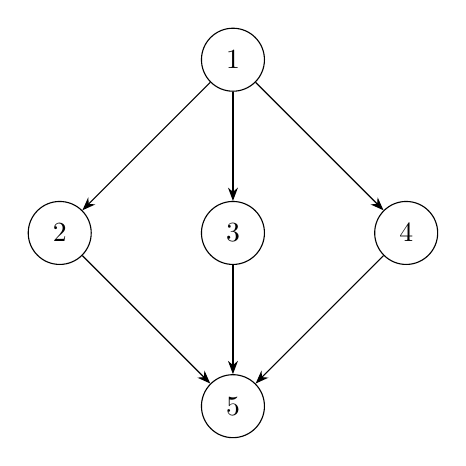
\begin{tikzpicture}[
  >=Stealth,
  every node/.style={circle, draw, minimum size=8mm, inner sep=0pt}
]
  \node (1) at (0, 2.2) {1};
  \node (2) at (-2.2, 0) {2};
  \node (3) at (0, 0) {3};
  \node (4) at (2.2, 0) {4};
  \node (5) at (0, -2.2) {5};
  \draw[->] (1) -- (2);
  \draw[->] (1) -- (3);
  \draw[->] (1) -- (4);
  \draw[->] (2) -- (5);
  \draw[->] (3) -- (5);
  \draw[->] (4) -- (5);
\end{tikzpicture}
\end{center}

\noindent
Directed edges: $1 \to 2$, $1 \to 3$, $1 \to 4$, $2 \to 5$, $3 \to 5$, $4 \to 5$.

\begin{enumerate}[label=\textbf{\alph*)}, leftmargin=*, itemsep=1em]

\item
Write the adjacency matrix $\mathbf{A}$ of the network (use the convention that entry $a_{ij}$ is equal to $1$ if node $j$ points to node $i$). Is matrix $\mathbf{A}$ symmetric?
\textbf{[4]}

\item
Determine the in-degree sequence $\{k_1^{\mathrm{in}}, k_2^{\mathrm{in}}, k_3^{\mathrm{in}}, k_4^{\mathrm{in}}, k_5^{\mathrm{in}}\}$ and the out-degree sequence $\{k_1^{\mathrm{out}}, k_2^{\mathrm{out}}, k_3^{\mathrm{out}}, k_4^{\mathrm{out}}, k_5^{\mathrm{out}}\}$ of the network. Find the nodes with the largest in-degree and the ones with the largest out-degree.
\textbf{[6]}

\item
Determine the in-degree distribution $P^{\mathrm{in}}(k)$ and the out-degree distribution $P^{\mathrm{out}}(k)$.
\textbf{[4]}

\item
State the definition of the Katz centrality $x_i$ of a node $i$ of a network. Find the Katz centrality for all the nodes of the network $G$.
\textbf{[7]}

\item
How many weakly and how many strongly connected components are there in the network $G$? Which are the nodes belonging to each one of these components?
\textbf{[3]}

\item
Consider now the underlying undirected network $G^{u}$ of $G$, i.e.\ the network obtained from $G$ by neglecting the directions of the links. Write the adjacency matrix $\mathbf{A}^{u}$ of $G^{u}$. How many links has network $G^{u}$?
\textbf{[4]}

\item
Write the $N \times N$ distance matrix $\mathbf{d}$ of network $G^{u}$ (remember that entry $d_{ij}$ indicates the length of the shortest paths between node $i$ and $j$). What is the diameter $D$ of $G^{u}$?
\textbf{[4]}

\item
Determine the degree distribution $P(k)$ of network $G^{u}$.
\textbf{[2]}

\item
State the definition of the betweenness centrality $b_i$ of a node $i$ of an undirected network. Evaluate the betweenness centrality $b_1$ of node $1$ and the betweenness centrality $b_4$ of node $4$ in network $G^{u}$.
\textbf{[6]}

\end{enumerate}

\end{document}
